\section{Phase 2 – Multimodal fusion with personalized emotion recognition}
\label{sec:exp-phase2}

This phase focuses on combining the selected models from Phase 1 to create a multimodal emotion recognition system. The goal is to enhance the accuracy and personalization of emotional state detection by integrating both facial and vocal data. The experimental flow for this phase is illustrated in Figure~\ref{fig:phase2}.

\begin{figure*}[h]
    \centering
    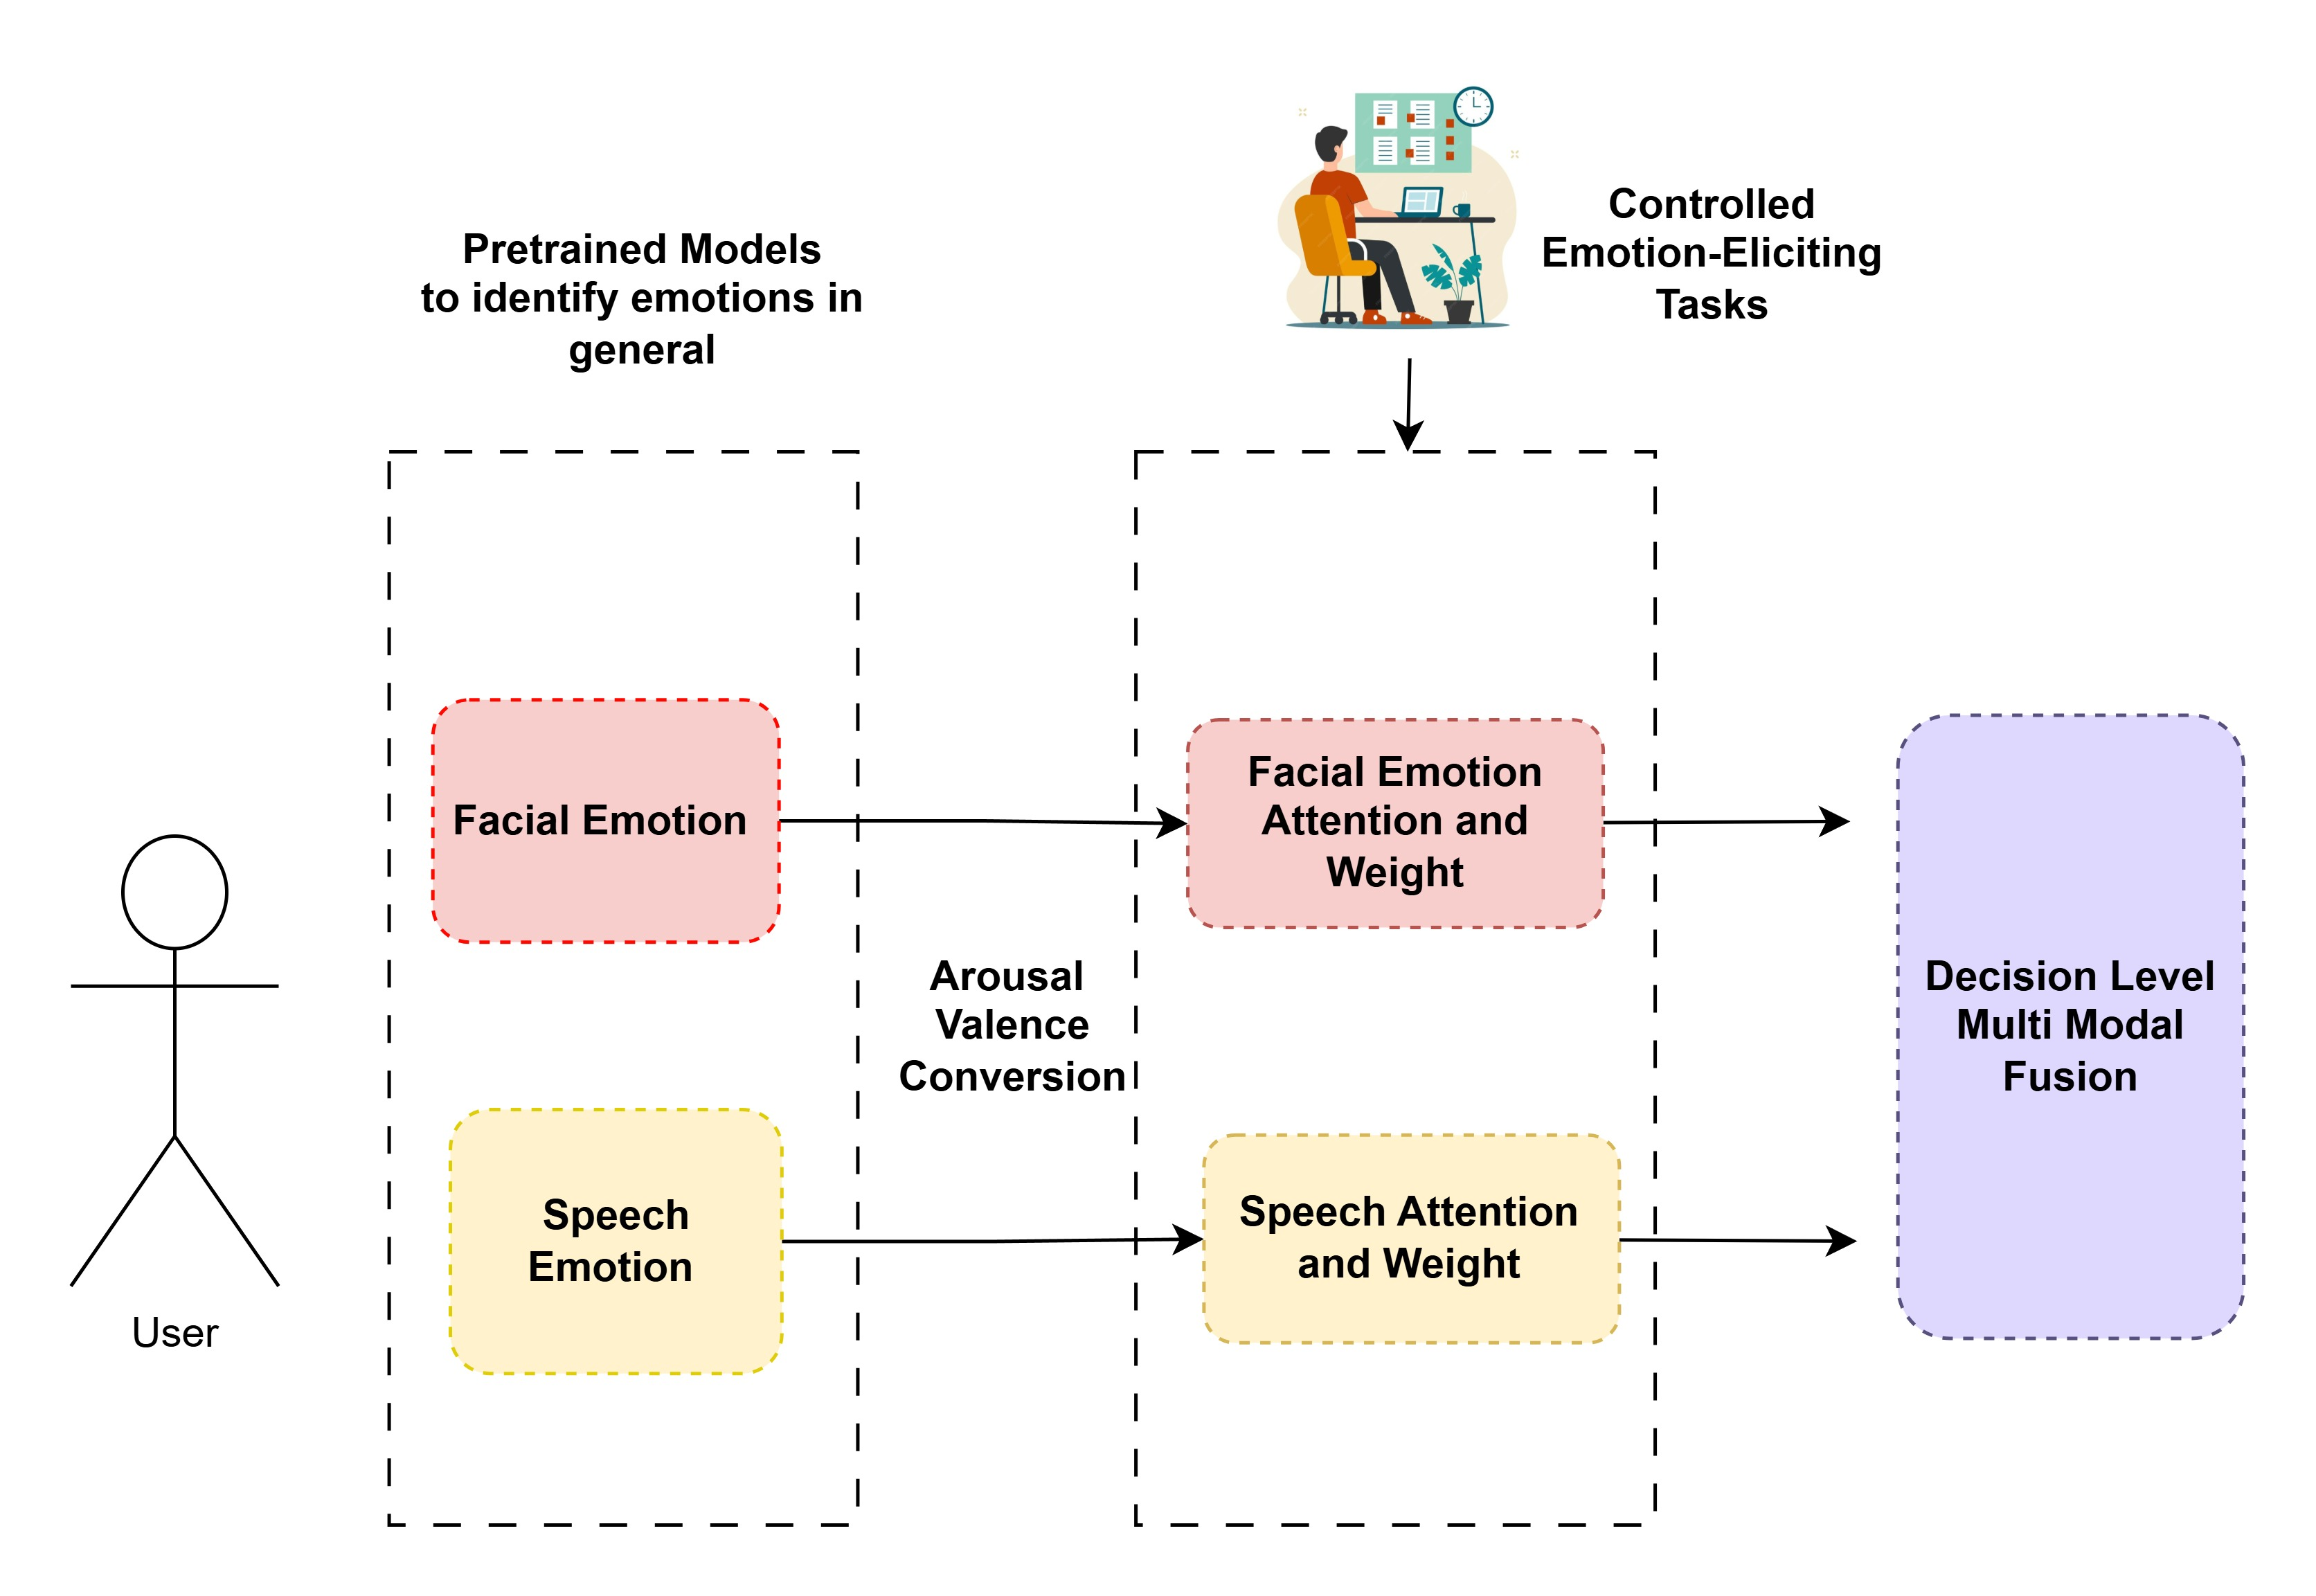
\includegraphics[width=1\textwidth]{img/chapter_03/Phase2.jpg}
    \captionof{figure}{Experimental flow of Phase 2}
    \label{fig:phase2}
\end{figure*}

\subsection{Emotion Eliciting Tasks}
\label{sec:eliciting-tasks}

In this phase, a set of emotion-eliciting tasks were designed to capture both facial and vocal expressions for five target emotions: \textbf{Happy, Angry, Sad, Boredom, and Calm}. These emotions were specifically chosen because they cover diverse directions in the Arousal-Valence (A-V) space, which helps in achieving better separation between emotional states. This separation allows the system to identify a clearer origin point for emotional detection, as illustrated in Figure~\ref{fig:av_isolation}.

\begin{figure*}[h]
    \centering
    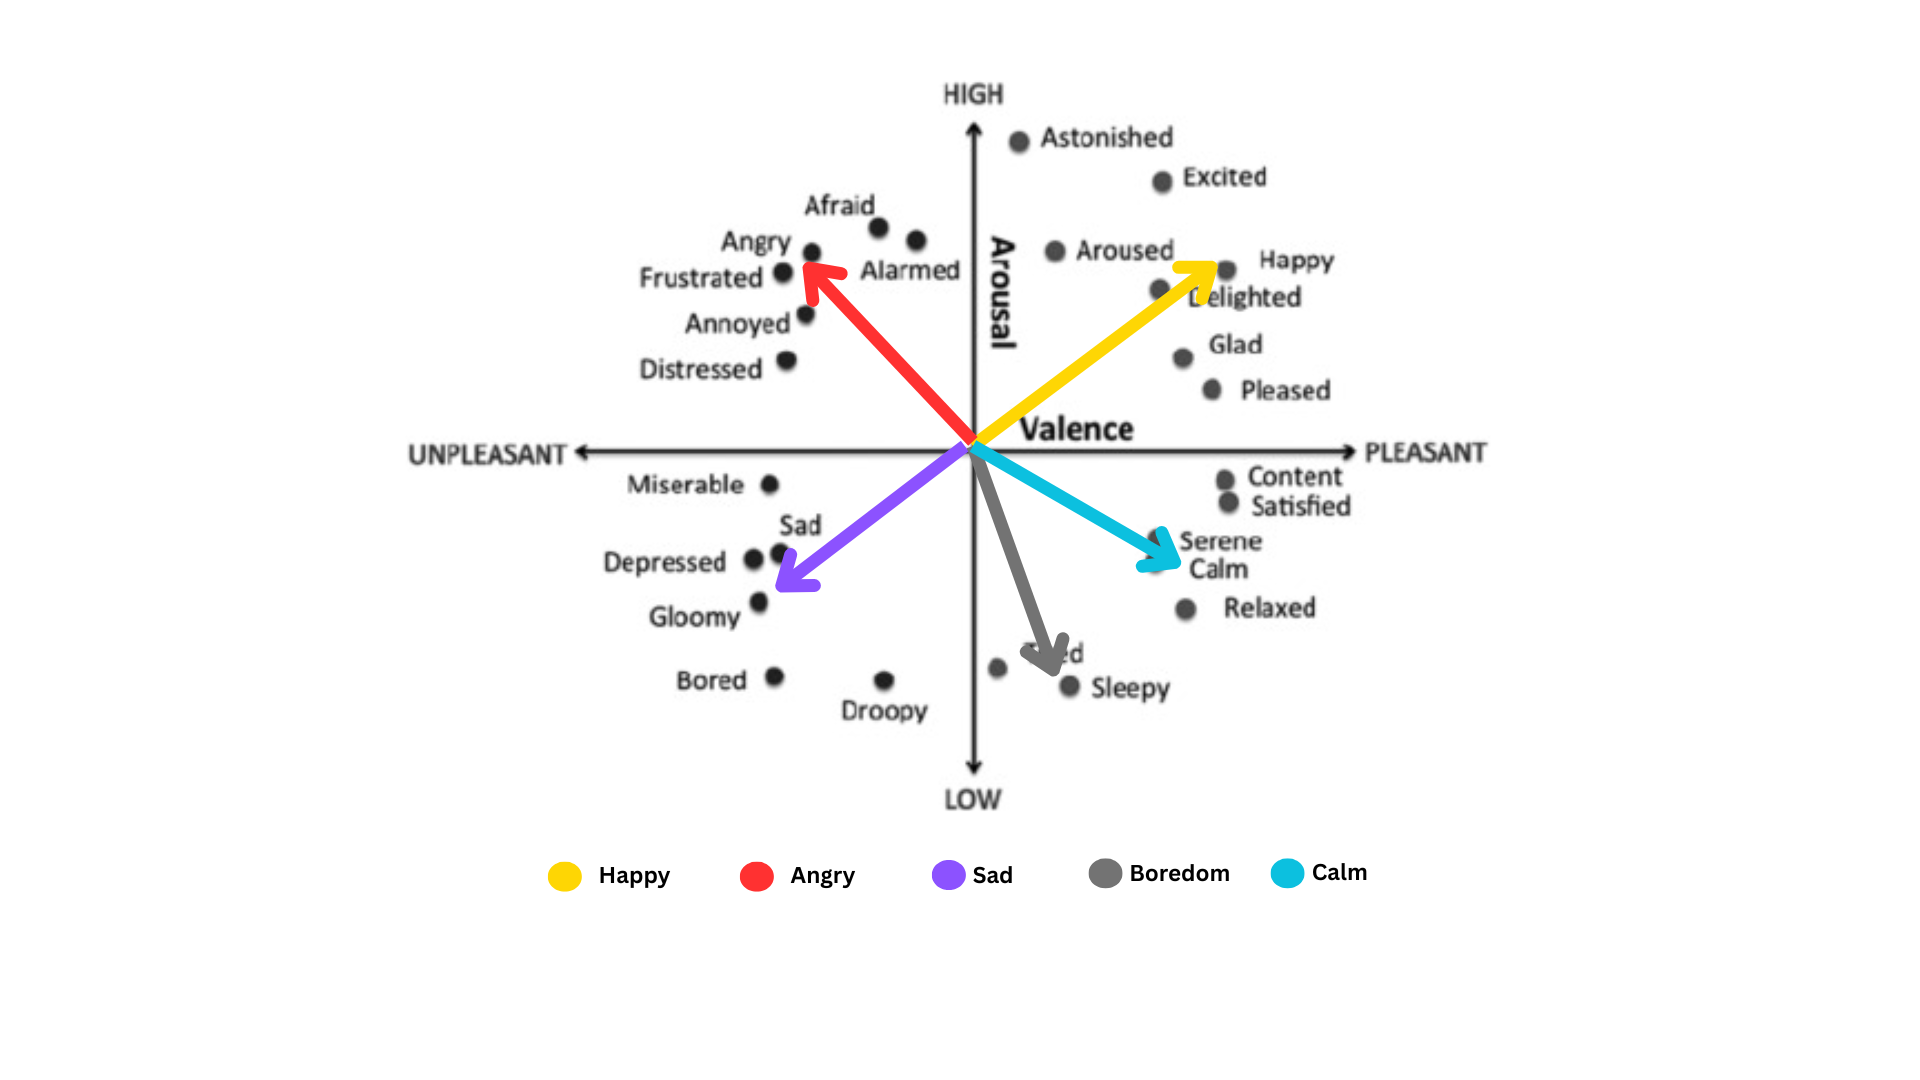
\includegraphics[width=1\textwidth]{img/chapter_03/elicting-tasks-av.png}
    \captionof{figure}{Arousal-Valence space with diverse emotion regions}
    \label{fig:av_isolation}
\end{figure*}

During the tasks, participants were asked to perform actions or respond to situations that naturally induce each of the five emotions. While they were doing the tasks, both facial expressions and vocal responses were recorded. The emotional points collected in this phase are later used in the next step to identify the user's emotional baseline.

As discussed in Section~\ref{sec:background}, emotions are highly personalized, and different people express them in unique ways. Therefore, to make the system more personalized, we combined the model outputs with user feedback. After each task, participants were asked to report how they actually felt and to rate the intensity of the emotion they experienced as shown in figure~\ref{fig:calm_eval}. This provided quantitative data directly from the user, which was used to adjust the emotion recognition output.

In addition, after collecting vocal expressions during each task, participants were briefly asked to describe how the experience felt in their own words. These voice recordings were used as extra vocal samples corresponding to that emotion.

At the end of the entire experiment, we also collected qualitative feedback from participants. While this feedback was not used to measure emotional levels, it gave valuable insights into how the system and tasks could be improved in future iterations of the research.


